\documentclass{article}

\usepackage{lipsum}
\usepackage[margin=1.2in]{geometry}
\usepackage{titlesec}
\usepackage{graphicx}
\usepackage{amsmath}

\newcommand{\code}{\texttt}
\newcommand{\norm}[1]{\left\lVert#1\right\rVert}

\usepackage{siunitx} % Required for alignment

\sisetup{
  round-mode          = places, % Rounds numbers
  round-precision     = 2, % to 2 places
}

% Specify images directory
\graphicspath{ {./report-images/} }

% Header and Footer stuff
\usepackage{fancyhdr}
\pagestyle{fancy}
\fancyhead{}
\fancyfoot{}
\fancyfoot[R]{ \thepage\ }
\renewcommand{\headrulewidth}{0pt}
\renewcommand{\footrulewidth}{0pt}
\newcommand{\sectionbreak}{\clearpage}
\setlength{\parindent}{0pt}

%

\begin{document}

%----------------------------------------------------------------------------------------
%	TITLE PAGE
%----------------------------------------------------------------------------------------

\begin{titlepage} % Suppresses displaying the page number on the title page and the subsequent page counts as page 1
	\newcommand{\HRule}{\rule{\linewidth}{0.5mm}}% Defines a new command for horizontal lines, change thickness here
	
	\center % Centre everything on the page
	
	%------------------------------------------------
	%	Headings
	%------------------------------------------------
	
	\textsc{\Large Systems of Linear Equations}\\[0.5cm] % Major heading such as course name
	
	\textsc{\large Exercise 7}\\[0.5cm] % Minor heading such as course title
	
	%------------------------------------------------
	%	Title
	%------------------------------------------------
	
	\HRule\\[0.6cm]
	
	{\huge\bfseries Solving a Linear System with LU Decomposition}\\[0.25cm] % Title of your document
	
	\HRule\\[1.5cm]
	
	%------------------------------------------------
	%	Author(s)
	%------------------------------------------------
	
	\begin{minipage}{0.4\textwidth}
		\begin{flushleft}
			\large
			\textit{Author}\\
			\textsc{Cesare De Cal} % Your name
		\end{flushleft}
	\end{minipage}
	~
	\begin{minipage}{0.4\textwidth}
		\begin{flushright}
			\large
			\textit{Professor}\\
			\textsc{Annie Cuyt}\\ % Supervisor's name
			[0.25cm]
			\textit{Assistant Professor}\\
			\textsc{Ferre Knaepkens} % Supervisor's name

		\end{flushright}
	\end{minipage}
		
	\vfill\vfill\vfill
	
	{\large\today}
		
	\vfill
	
\end{titlepage}

%----------------------------------------------------------------------------------------

\section{Introduction}\label{sec:intro}
This exercise asks to build a tridiagonal matrix with the value $-1$ on the adjacent upper diagonal, the value $+1$ on the adjacent lower diagonal, and the value $b_{i}$ on the main diagonal, with $i = 1, \ldots, n$ given by
$$b_i =\frac{2(i+1)}{3},\quad i + 1= 3, 6, 9,\ldots$$
$$b_i =1,\quad i + 1 = 2, 4, 5, 7, 8, \ldots$$

This matrix should then be used as the coefficients matrix in the $A\vec{x}=\vec{y}$ linear system. The exercise asks to solve the system using \code{GEPP} (Gaussian Elimination with Partial Pivoting) and then give $x_1$, which should be an approximation of the $e-2$.\\

As we've seen in class, there are multiple ways of solving a linear system. For example, we could compute the inverse of $A$ and find $\vec{x}=A^{-1}\vec{y}$. We've seen that this approach, however, requires more computations than necessary and returns a less accurate result. Therefore in this exercise I am going to use solve a linear system using LU decomposition.\\

LU decomposition, used to represent the matrix A in the form of simpler matrices, $L$ and $U$ (lower triangular and upper triangular matrices, respectively), uses forward substitution (solving for $Y$ from $LY=B$) and backward substitution (solving for $X$ from $UX = Y$). As seen in class, this method is numerically stable (as in, there will be no extra truncation errors). I'll also be calculating the condition number and the error to verify if this is an ill-conditioned system and to verify how precise the computed solution is.

\section{Tools}
The following programming language and libraries have been used in this exercise:
\begin{itemize}
  \item C
  \item GSL (GNU Scientific Library)
\end{itemize}
The following double-precision GSL data types have been used in the exercise:
\begin{itemize}
  \item \code{gsl\_vector}
  \item \code{gsl\_matrix}
  \item \code{gsl\_permutation}
\end{itemize}
The following GSL methods have been used in the exercise:
\begin{itemize}
  \item \code{gsl\_matrix\_alloc(size1, size2)}
  \item \code{gsl\_matrix\_set\_zero(matrix)}
  \item \code{gsl\_matrix\_set(matrix, row, column, value)}
  \item \code{gsl\_matrix\_get(matrix, row, column)}
  \item \code{gsl\_vector\_alloc(size)}
  \item \code{gsl\_vector\_set\_zero(vector)}
  \item \code{gsl\_vector\_set(vector, index, value)}
  \item \code{gsl\_vector\_get(vector, index)}
  \item \code{gsl\_matrix\_memcpy(matrixToCopyFrom, matrix)}
  \item \code{gsl\_linalg\_SV\_decomp(A, V, S, workspaceVector)}
  \item \code{gsl\_vector\_minmax(vector, minInVector, maxInVector)}
\end{itemize}
In order to factorize a matrix into the LU decomposition, and then solve the square system $Ax=y$ using the decomposition of A, I've used the following methods:
\begin{itemize}
  \item \code{gsl\_linalg\_LU\_decomp(A, permutation, signum)}
  \item \code{gsl\_linalg\_LU\_solve(LU, permutation, b, x)}
  \item \code{gsl\_permutation\_alloc(size)}
\end{itemize}
  
\section{Solving the Linear System}
By looking closely at the first rule, we see that the $i+1$ are all multiples of 3 ($i+1 = 3*k$, for some $k$). Hence the $i$ are of the form $i = 3*k-1$, for some $k$. For $n = 5$, for example, this is what the coefficient matrix looks like:
$$
\begin{bmatrix}
1.000000000e+00 & -1.000000000e+00 & 0.000000000e+00 & 0.000000000e+00 & 0.000000000e+00 \\ 
1.000000000e+00 & 2.000000000e+00 & -1.000000000e+00 & 0.000000000e+00 & 0.000000000e+00 \\ 
0.000000000e+00 & 1.000000000e+00 & 1.000000000e+00 & -1.000000000e+00 & 0.000000000e+00 \\ 
0.000000000e+00 & 0.000000000e+00 & 1.000000000e+00 & 1.000000000e+00 & -1.000000000e+00 \\ 
0.000000000e+00 & 0.000000000e+00 & 0.000000000e+00 & 1.000000000e+00 & 4.000000000e+00 \\
\end{bmatrix}
$$

The coefficients matrix A is first allocated by using the \code{gsl\_matrix\_alloc} method, then I set all the elements to zero with \code{gsl\_matrix\_set\_zero} and finally nested \code{for} loops fill the diagonal values by checking the indexes. The coefficients reported above on the diagonal have 5 significant digits for improve the readability of this report.\\

I used the \code{gsl\_vector\_alloc} method to create an instance of the vector. All of its elements were set to zero by using \code{gsl\_vector\_set\_zero(vector)}. The exercise asks us to set the first element of the $y$ vector to one, so I used \code{gsl\_vector\_set(vector, 0, 1)} to assign the value 1 to index 0. For $n=5$, we have:
$$
\vec{y}=
\begin{bmatrix}
1.000000000e+00 \\
0.000000000e+00 \\
0.000000000e+00 \\
0.000000000e+00 \\
0.000000000e+00 \\
\end{bmatrix}
$$

Given the $Ax=y$ system, my goal is now to find the vector of the unknowns $x$. To do so, I first factorize $A$ into its LU decomposition by allocating a new matrix (so that the matrix which represents $A$ doesn't get overridden) using \code{gsl\_matrix\_memcpy} and then by calling \code{gsl\_linalg\_LU\_decomp}. This method utilizes Gaussian Elimination with partial pivoting to compute the decomposition. The following is the $LU$ matrix for $n=5$:
$$
\begin{bmatrix} 
1.000000000e+00 & -1.000000000e+00 & 0.000000000e+00 & 0.000000000e+00 & 0.000000000e+00 \\ 
1.000000000e+00 & 3.000000000e+00 & -1.000000000e+00 & 0.000000000e+00 & 0.000000000e+00 \\ 
0.000000000e+00 & 3.333333333e-01 & 1.333333333e+00 & -1.000000000e+00 & 0.000000000e+00 \\
0.000000000e+00 & 0.000000000e+00 & 7.500000000e-01 & 1.750000000e+00 & -1.000000000e+00 \\ 
0.000000000e+00 & 0.000000000e+00 & 0.000000000e+00 & 5.714285714e-01 & 4.571428571e+00 \\
\end{bmatrix}
$$

I can now use the $LU$ matrix to solve the system by passing $LU$, $x$, a permutation structure \code{gsl\_permutation} (it contains the order of the indexes of the equations in the system to keep track of swapping) and $y$ to \code{gsl\_linalg\_LU\_solve}. This method uses forward and back-substitution to modify the contents of the $x$ vector given in input, which now looks like this (for $n=5$):

$$
\vec{x}=
\begin{bmatrix}
7.187500000e-01\\
-2.812500000e-01\\
1.562500000e-01\\
-1.250000000e-01\\
3.125000000e-02\\
\end{bmatrix}
$$

Then, I calculate the condition number of the matrix $A$ of order $n$ which will give me a better idea if this is a well-conditioned or an ill-conditioned linear system. In GSL there is no direct function that calculates the condition number, but it's possible to use the ratio of the largest singular value of matrix A, $\sigma_n (A)$, to the smallest $\sigma_1 (A)$:

$$\kappa(A) := \frac{\sigma_n (A)}{\sigma_1 (A)}= \frac{\norm{A}}{\norm{A^{-1}}^{-1}}$$

I proceed to factorize $A$ into its singular value decomposition $SVD$ using the \code{gsl\_linalg\_SV\_decomp} method, and then use $\code{gsl\_vector\_minmax}$ to extract the minimum and maximum singular values out of the vector $S$ that contains the diagonal elements of the singular value matrix. \\

For $n=5$, the condition number is

$$\kappa(A) = \frac{\sigma_n (A)}{\sigma_1 (A)}= \frac{4.205100611e+00}{1.142643287e+00}=3.680151678e+00$$

I calculate the error by subtracting the computed solution $x_{1}^{\ast}$ from the exact mathematical solution $\widetilde{x}$ (which can be obtained by using the $\code{M\_E}$ GSL constant minus 2).\\

\begin{table*}[htb]
\centering % used for centering table
\begin{tabular}{c c c c} % centered columns (4 columns)
$n$ & $\widetilde{x}_1$ & $x_1^{\ast}- \widetilde{x}_1$ & $\kappa(A_n)$ \\ [0.65ex] % inserts table
%heading
\hline % inserts single horizontal line
1 & 1.000000000e+00 & -2.817181715e-01 & 1.000000000e+00 \\
2 & 6.666666667e-01 & 5.161516179e-02 & 1.767591879e+00 \\
3 & 7.500000000e-01 & -3.171817154e-02 & 2.561552813e+00 \\
4 & 7.142857143e-01 & 3.996114173e-03 & 2.258696038e+00 \\
5 & 7.187500000e-01 & -4.681715410e-04 & 3.680151678e+00 \\
6 & 7.179487179e-01 & 3.331105103e-04 & 3.953864002e+00 \\
7 & 7.183098592e-01 & -2.803069588e-05 & 3.847674609e+00 \\
8 & 7.182795699e-01 & 2.258566572e-06 & 5.377037588e+00 \\
9 & 7.182835821e-01 & -1.753630507e-06 & 5.727581839e+00 \\
10 & 7.182817183e-01 & 1.101773268e-07 & 5.498872833e+00 \\
11 & 7.182818352e-01 & -6.746947445e-09 & 7.100335770e+00 \\
12 & 7.182818229e-01 & 5.515095380e-09 & 7.582164638e+00 \\
13 & 7.182818287e-01 & -2.766507023e-10 & 7.195531702e+00 \\
14 & 7.182818284e-01 & 1.364375279e-11 & 8.833149892e+00 \\
15 & 7.182818285e-01 & -1.153854789e-11 & 9.488074730e+00 \\
16 & 7.182818285e-01 & 4.816147481e-13 & 8.911558696e+00 \\
17 & 7.182818285e-01 & -1.998401444e-14 & 1.057152285e+01 \\
18 & 7.182818285e-01 & 1.709743458e-14 & 1.142018246e+01 \\
19 & 7.182818285e-01 & -6.661338148e-16 & 1.063813407e+01 \\
20 & 7.182818285e-01 & -1.110223025e-16 & 1.231319966e+01 \\
21 & 7.182818285e-01 & -2.220446049e-16 & 1.336883104e+01 \\
22 & 7.182818285e-01 & -2.220446049e-16 & 1.237107821e+01 \\
23 & 7.182818285e-01 & -2.220446049e-16 & 1.405700479e+01 \\
24 & 7.182818285e-01 & -2.220446049e-16 & 1.532862983e+01 \\
25 & 7.182818285e-01 & -2.220446049e-16 & 1.410816377e+01 \\
26 & 7.182818285e-01 & -2.220446049e-16 & 1.580226249e+01 \\
27 & 7.182818285e-01 & -2.220446049e-16 & 1.729630706e+01 \\
28 & 7.182818285e-01 & -2.220446049e-16 & 1.584809348e+01 \\
29 & 7.182818285e-01 & -2.220446049e-16 & 1.754855617e+01 \\
30 & 7.182818285e-01 & -2.220446049e-16 & 1.926975724e+01 \\
31 & 7.182818285e-01 & -2.220446049e-16 & 1.759006043e+01 \\
32 & 7.182818285e-01 & -2.220446049e-16 & 1.929561485e+01 \\
33 & 7.182818285e-01 & -2.220446049e-16 & 2.124756325e+01 \\
34 & 7.182818285e-01 & -2.220446049e-16 & 1.933353645e+01 \\
35 & 7.182818285e-01 & -2.220446049e-16 & 2.104325456e+01 \\
36 & 7.182818285e-01 & -2.220446049e-16 & 2.322873622e+01 \\
37 & 7.182818285e-01 & -2.220446049e-16 & 2.107816128e+01 \\
38 & 7.182818285e-01 & -2.220446049e-16 & 2.279134599e+01 \\
39 & 7.182818285e-01 & -2.220446049e-16 & 2.521256520e+01 \\
40 & 7.182818285e-01 & -2.220446049e-16 & 2.282368084e+01 \\
41 & 7.182818285e-01 & -2.220446049e-16 & 2.453979556e+01 \\
42 & 7.182818285e-01 & -2.220446049e-16 & 2.719852600e+01 \\
43 & 7.182818285e-01 & -2.220446049e-16 & 2.456991077e+01 \\
44 & 7.182818285e-01 & -2.220446049e-16 & 2.628853390e+01 \\
45 & 7.182818285e-01 & -2.220446049e-16 & 2.918622370e+01 \\
46 & 7.182818285e-01 & -2.220446049e-16 & 2.631671410e+01 \\
47 & 7.182818285e-01 & -2.220446049e-16 & 2.803750846e+01 \\
48 & 7.182818285e-01 & -2.220446049e-16 & 3.117535515e+01 \\
49 & 7.182818285e-01 & -2.220446049e-16 & 2.806398692e+01 \\
50 & 7.182818285e-01 & -2.220446049e-16 & 2.978667872e+01 \\\hline %inserts single line
\end{tabular}
\end{table*}

\section{Plot}
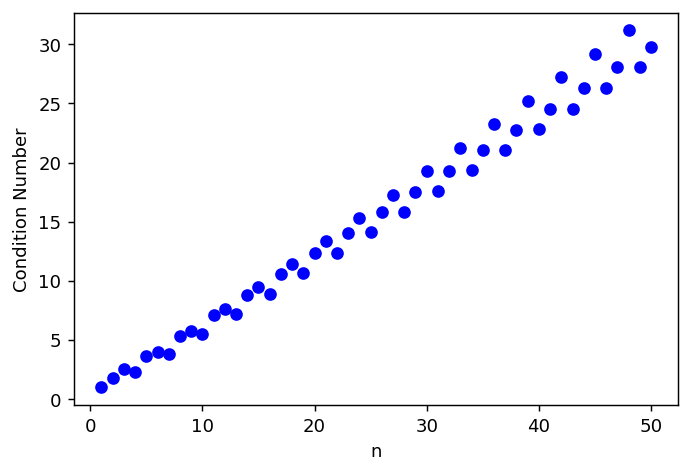
\includegraphics[width=\textwidth,height=\textheight,keepaspectratio]{cond_number.png}

\section{Observations}
The linear system presented in this exercise gets increasingly ill-conditioned as $n$ grows (since $\kappa(A_n)> 1$ for most $n$). From the plot, it can be observed that the condition number grows linearly. It can be noticed, however, that a large condition number doesn’t necessarily mean that the error will be large in all cases, just that it is possible to have a large error. However, it can be observed that as $n$ increases, the error gets incrementally smaller.\\

The error that I have calculated represents how well the computed solution $\widetilde{x}_1$ approximates the true solution $x_1^{\ast}$. It can be noted that the Gaussian elimination with partial pivoting doesn't introduce any additional truncation errors and therefore it is numerically stable.

\end{document}